\documentclass[tikz, border=5mm]{standalone}
\usepackage{pgfplots}
\pgfplotsset{compat=1.18} % Use a recent pgfplots compatibility mode

\begin{document}
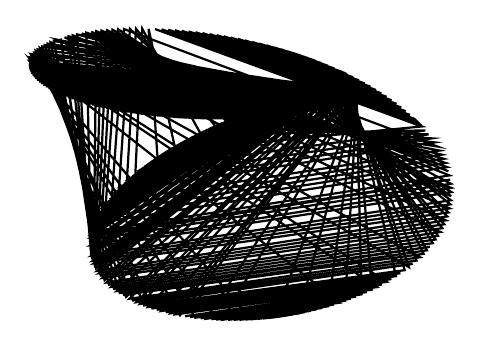
\begin{tikzpicture}
  \begin{axis}[
    view={-70}{35}, % Viewing angle (azimuth, elevation)
    axis lines=none, % Hide the x, y, z axes, ticks, and labels
    z buffer=sort,   % Ensures correct drawing order for 3D elements
    clip=false       % Allows elements to extend slightly outside the axis box
  ]

  % Parameters for the Mobius strip
  \def\R{2.5} % Major radius of the strip's "core" circle
  \def\w{0.8} % Half-width of the strip

  % Contour (edge) of the Mobius strip
  % This is a single continuous curve.
  % Parametrization:
  % x(u) = (R + w*cos(u/2)) * cos(u)
  % y(u) = (R + w*cos(u/2)) * sin(u)
  % z(u) = w*sin(u/2)
  % where u goes from 0 to 720 degrees (4*pi radians) to trace the entire edge.
  \addplot3[
    color=black,      % Color of the contour line
    thick,            % Thickness of the contour line
    samples=400,      % Number of samples for a smooth curve (increased for smoothness of the single edge)
    domain=0:720,     % Parameter u from 0 to 720 degrees for the full edge
    variable=\u,      % Name of the parameter
    samples y=0,      % Important hint for pgfplots that this is a line, not a surface
  ]
  ( % Parametric equations for x, y, z coordinates of the edge
    {(\R + \w*cos(\u/2)) * cos(\u)}, % x(u)
    {(\R + \w*cos(\u/2)) * sin(\u)}, % y(u)
    {\w*sin(\u/2)}                   % z(u)
  );

  \end{axis}
\end{tikzpicture}
\end{document}
